% This is "sig-alternate.tex" V2.0 May 2012
% This file should be compiled with V2.5 of "sig-alternate.cls" May 2012
%
% This example file demonstrates the use of the 'sig-alternate.cls'
% V2.5 LaTeX2e document class file. It is for those submitting
% articles to ACM Conference Proceedings WHO DO NOT WISH TO
% STRICTLY ADHERE TO THE SIGS (PUBS-BOARD-ENDORSED) STYLE.
% The 'sig-alternate.cls' file will produce a similar-looking,
% albeit, 'tighter' paper resulting in, invariably, fewer pages.
%
% ----------------------------------------------------------------------------------------------------------------
% This .tex file (and associated .cls V2.5) produces:
%       1) The Permission Statement
%       2) The Conference (location) Info information
%       3) The Copyright Line with ACM data
%       4) NO page numbers
%
% as against the acm_proc_article-sp.cls file which
% DOES NOT produce 1) thru' 3) above.
%
% Using 'sig-alternate.cls' you have control, however, from within
% the source .tex file, over both the CopyrightYear
% (defaulted to 200X) and the ACM Copyright Data
% (defaulted to X-XXXXX-XX-X/XX/XX).
% e.g.
% \CopyrightYear{2007} will cause 2007 to appear in the copyright line.
% \crdata{0-12345-67-8/90/12} will cause 0-12345-67-8/90/12 to appear in the copyright line.
%
% ---------------------------------------------------------------------------------------------------------------
% This .tex source is an example which *does* use
% the .bib file (from which the .bbl file % is produced).
% REMEMBER HOWEVER: After having produced the .bbl file,
% and prior to final submission, you *NEED* to 'insert'
% your .bbl file into your source .tex file so as to provide
% ONE 'self-contained' source file.
%
% ================= IF YOU HAVE QUESTIONS =======================
% Questions regarding the SIGS styles, SIGS policies and
% procedures, Conferences etc. should be sent to
% Adrienne Griscti (griscti@acm.org)
%
% Technical questions _only_ to
% Gerald Murray (murray@hq.acm.org)
% ===============================================================
%
% For tracking purposes - this is V2.0 - May 2012

\documentclass{sig-alternate}
\usepackage[T1]{fontenc}
\usepackage[utf8]{inputenc}
\usepackage{algorithm,caption,algpseudocode}
\usepackage{color}
%\usepackage[round]{natbib}
\usepackage{hyperref}
\usepackage{multicol}

\newcommand\alert[1]{\textcolor{red}{#1}}
\newcommand\note[1]{\textcolor{blue}{#1}}
\newcommand\jb[1]{\textcolor{green!50!black}{#1}}

\begin{document}
%
% --- Author Metadata here ---
\conferenceinfo{L@S 2015,}{March 14 -- 15 2015, Vancouver, BC, USA}
%\CopyrightYear{2007} % Allows default copyright year (20XX) to be over-ridden - IF NEED BE.
%\crdata{0-12345-67-8/90/01}  % Allows default copyright data (0-89791-88-6/97/05) to be over-ridden - IF NEED BE.
% --- End of Author Metadata ---

\title{\note{Predicting Performance on Binary Questions:\\Comparing Models for Large-Scale Adaptive Testing}}
%\subtitle{An exhaustive survey}
%
% You need the command \numberofauthors to handle the 'placement
% and alignment' of the authors beneath the title.
%
% For aesthetic reasons, we recommend 'three authors at a time'
% i.e. three 'name/affiliation blocks' be placed beneath the title.
%
% NOTE: You are NOT restricted in how many 'rows' of
% "name/affiliations" may appear. We just ask that you restrict
% the number of 'columns' to three.
%
% Because of the available 'opening page real-estate'
% we ask you to refrain from putting more than six authors
% (two rows with three columns) beneath the article title.
% More than six makes the first-page appear very cluttered indeed.
%
% Use the \alignauthor commands to handle the names
% and affiliations for an 'aesthetic maximum' of six authors.
% Add names, affiliations, addresses for
% the seventh etc. author(s) as the argument for the
% \additionalauthors command.
% These 'additional authors' will be output/set for you
% without further effort on your part as the last section in
% the body of your article BEFORE References or any Appendices.

\numberofauthors{4} %  in this sample file, there are a *total*
% of EIGHT authors. SIX appear on the 'first-page' (for formatting
% reasons) and the remaining two appear in the \additionalauthors section.
%
\author{
% You can go ahead and credit any number of authors here,
% e.g. one 'row of three' or two rows (consisting of one row of three
% and a second row of one, two or three).
%
% The command \alignauthor (no curly braces needed) should
% precede each author name, affiliation/snail-mail address and
% e-mail address. Additionally, tag each line of
% affiliation/address with \affaddr, and tag the
% e-mail address with \email.
%
% 1st. author
\alignauthor \phantom{Jill-Jênn Vie}%
       \affaddr{\phantom{ENS Cachan -- Bât. Cournot}}%
       \affaddr{\phantom{61 av. du Président Wilson}}%
       \affaddr{\phantom{94235 Cachan, France}}%
%       \email{\phantom{vie@jill-jenn.net}}%
% 2nd. author
\alignauthor
\phantom{Fabrice Popineau}
       \affaddr{\phantom{Supélec -- Dép. informatique}}
       \affaddr{\phantom{3 rue Joliot Curie}}
       \affaddr{\phantom{91192 Gif-sur-Yvette, France}}
%       \email{\phantom{fabrice.popineau@supelec.fr}}
% 3rd. author
\alignauthor
\phantom{Jean-Bastien Grill}
       \affaddr{\phantom{École normale supérieure}}
       \affaddr{\phantom{45 rue d'Ulm}}
       \affaddr{\phantom{75005 Paris}}
%       \email{\phantom{grill@clipper.ens.fr}}
\and
% 4th. author
\alignauthor \phantom{Éric Bruillard}
       \affaddr{\phantom{ENS Cachan -- Bât. Cournot}}
       \affaddr{\phantom{61 av. du Président Wilson}}
       \affaddr{\phantom{94235 Cachan, France}}
       \email{\phantom{eric.bruillard@ens-cachan.fr}}
% 5th. author
\alignauthor
\phantom{Yolaine Bourda}
       \affaddr{\phantom{Supélec -- Dép. informatique}}
       \affaddr{\phantom{3 rue Joliot Curie}}
       \affaddr{\phantom{91192 Gif-sur-Yvette, France}}
       \email{\phantom{yolaine.bourda@supelec.fr}}
}
% There's nothing stopping you putting the seventh, eighth, etc.
% author on the opening page (as the 'third row') but we ask,
% for aesthetic reasons that you place these 'additional authors'
% in the \additional authors block, viz.
% \additionalauthors{Additional authors: John Smith (The Th{\o}rv{\"a}ld Group,
% email: {\texttt{jsmith@affiliation.org}}) and Julius P.~Kumquat
% (The Kumquat Consortium, email: {\texttt{jpkumquat@consortium.net}}).}
\date{October 29, 2014}
% Just remember to make sure that the TOTAL number of authors
% is the number that will appear on the first page PLUS the
% number that will appear in the \additionalauthors section.

\maketitle
\begin{abstract}
Computerized adaptive testing (CAT) is a mode of testing which has gained increasing popularity over the past years. It selects the questions asked to the examinee in order to evaluate her level efficiently, by using her answers to the previous questions.
Traditionally, CAT systems have been relying on item response theory (IRT) in order to provide an effective measure of latent abilities in possibly large-scale assessments.
More recently, from the perspective of providing useful feedback to examinees, other models have been studied for cognitive diagnosis. One of them is q-matrices, drawing a link between questions and examinee skills.
In this paper, we define a protocol to evaluate adaptive testing algorithms that enables us to use q-matrices in the context of assessments and to compare them to item response theory.
\note{Results made on a real dataset of 58,939 of sixth- and seventh-grade students suggest that although it is a simpler model, IRT is slightly better than q-matrices at predicting student answers.}
\end{abstract}

% A category with the (minimum) three required fields
\category{}{Student assessment}{Adaptive testing}
%A category including the fourth, optional field follows...

\terms{Q-matrices, computerized adaptive testing, item response theory}

\keywords{Adaptive assessment, computerized adaptive testing, cognitive diagnosis, item response theory, q-matrices}

\newpage

\section{Introduction}
Automated assessment of student answers has recently gained popularity in the context of online initiatives such as the GMAT~\cite{Rudner2010}, or massive online open courses (MOOCs). Such systems must be able to rank thousands of students for evaluation or recruiting purposes and to provide personal feedback automatically \alert{for} formative purposes.

If we already have a large-scale database of item responses for a certain test, it is natural to wonder which questions yield the most information about an examinee, i.e. if there is a ``best'' order in which the questions should be asked. In oral examinations, the examiner usually picks the next question to ask according to the previous answers of the examinee. Computerized adaptive testing (CAT) can be seen as an automated version of this process: keep asking the \alert{most useful} questions until enough information has been gathered. Indeed, if the examinee behaves typically, a subset of carefully chosen results may be enough to guess how she will perform on the rest of the questions.

In order to fulfill this need, item response theory (IRT) is of great help. The initial purpose of IRT was to provide a framework to evaluate the performance of individual questions, called \emph{items}, on assessments~\cite{Hambleton1991}. It has been successfully applied to computerized adaptive testing and several methods have been proposed and implemented. According to her performance, an examinee gets a summative score, making it possible to predict her future answers. The simplicity of the IRT models both made it amenable to theoretical analysis~\cite{Baker2004} and further increased its popularity.

More recently, the No Child Left Behind Act of 2001 called for more formative assessments, putting emphasis on the early detection of students with cognitive disabilities and urged the need of cognitive diagnosis models. Instead of a summative score, examinees would receive a detailed feedback, specifying which skills are mastered and which ones are not~\cite{Cheng2009}. These models allow researchers to reveal possible misconceptions of the examinee in order to propose appropriate exercises. Most of these models rely on a q-matrix specifying for each question the different skills required to solve it. For example, a fraction test may require 1) converting a whole number to a fraction, 2) separating a whole number from a fraction, 3) simplifying before subtracting, and so on~\cite{DeLaTorreDouglas2004}. Cognitive diagnosis adaptive tests have been designed in order to guess the skills of the examinee effectively~\cite{Huebner2010}.

One could wonder why we compare a model designed for evaluation with a model designed for feedback. We show that although the q-matrix model were first designed for formative assessments, it is also possible to use it in the context of large-scale assessments. Indeed, this model evaluates the skills of an examinee according to her previous answers. Given those computed skills and the q-matrix, we can predict her probability of correctly answering the remaining questions. This enables us to propose a protocol for comparison that captures both models.

Originally, q-matrices were specified by experts, but recent work in the educational data mining field attempts to infer q-matrices directly from student data~\cite{Huebner2010}. The corresponding skills are therefore implicit, but such automatically extracted q-matrices have proven to produce better inference~\cite{Barnes2003}.

\subsection{Our Contribution}

In this paper, we propose a new protocol to evaluate adaptive testing algorithms and use it to compare the performances of both a traditional CAT using \alert{the Rasch model from} item response theory and a more recent cognitive diagnosis model from the literature in psychometrics using q-matrices. More precisely, we expect to answer the following question: given a budget of $B$ questions asked according to a certain adaptive selection rule, which model performs the best in predicting the answers of the examinee over the remaining questions? To the best of our knowledge, no such comparison has ever been made.

Whereas the Rasch model is the most commonly used \note{model} for adaptive testing, q-matrices are an useful tool for fine-grained cognitive diagnosis. Our results show that the Rasch model is slightly better than our implementation of q-matrix.

\subsection{Outline}

We first present the computerized adaptive testing framework and two models chosen respectively from item response theory and cognitive diagnosis research. We then detail the design of these models and the proposed \alert{protocol} to evaluate them in our simulation. Finally, we present our results.

\section{Background and Related Work}

\subsection{Computerized Adaptive Testing}

In a computerized adaptive test (CAT), the examinee is presented with adaptively selected questions according to her previous performance. Thus, a CAT framework relies on two main subroutines:
\begin{itemize}
\item \textsc{NextItem}: the item selection algorithm, that picks the next question to ask according to the previous answers of the examinee;
\item \textsc{TerminationRule}: a condition that will end the test, when enough information has been gathered and the competence has been measured satisfyingly.
\end{itemize}

The framework of a CAT can be represented by the following algorithm: while the termination rule is not satisfied, the algorithm picks the question that optimizes a certain criterion according to the item selection rule.

Common criteria for the item selection rule are maximizing the Fisher information of \alert{the system}, minimizing the Shannon entropy of the distribution over the parameters, or maximizing the Kullback-Leibler divergence~\cite{Xu2003}. % TOFIX

\subsection{Item Response Theory}

For our needs, IRT provides a commonly used model allowing to compute the probability of answering correctly each question. Basically, the Rasch model estimates the latent ability of a student by a unique real number $\theta$ modeled by a random variable and characterizes each question by two real numbers:

\begin{itemize}
\item the \emph{difficulty} $d$, corresponding to the ability needed to answer the question correctly;
\item the \emph{discrimination} $\delta$, representing the capacity of the question to draw a separation between students that have the required ability from those that do not.
\end{itemize}

Knowing the hidden ability $\theta_i$ of a given student $i$, the difficulty $d_j$ and the discrimination parameter $\delta_j$ of a given question $j$, the probability of the event ``the student $i$ answers correctly the question $j$'', which we denote \alert{hereafter} by \emph{success}$_{ij}$, is modeled by:
\[ \Pr\{success_{ij}|\theta_i\} = \frac1{1+e^{-\delta_j(\theta_i - d_j)}}. \]

The aim is first to optimize the parameters $d_j$, $\delta_j$ for each question $j$ and $\theta_i$ for each student $i$ in order to fit a given train dataset. Then, during the CAT process, a probability distribution over $\theta_i$ is maintained and each question answered allows to refine the confidence interval around $\theta_i$ using the Bayes' rule. The probability of \emph{success}$_{ij}$ knowing the parameters can thus be computed by integrating over the hidden variable $\theta_i$.

\[ \Pr\{success_{ij}\} = \int \Pr\{success_{ij}|\theta_i\} \Pr\{\theta_i\} \mathrm d\theta_i \]

This simple model is used in computerized adaptive testing, where many methods are implemented for next item selection~\cite{MagisRaiche2012}. \note{Some extensions exist such as multidimensional item response theory but their complexity is much greater~\cite{Desmarais2012} and they are harder to train. The SPARFA model for test-size reduction developed in~\cite{Vats2013} is itself a variant of the MIRT model, where coefficients are limited to nonnegative values.}

\subsection{Cognitive Diagnosis Model}

The Rasch model we just described uses a single parameter to represent students. We now develop a model that tries to be more informative about the student skills. Every student is modeled by a vector of binary values $(a_1, \ldots, a_K)$, called \emph{skill vector}, representing her mastery of $K$ different skills, thus leading to $2^K$ possible skill vectors. 

A q-matrix $Q$ \cite{Tatsuoka1983} represents the different skills involved in answering every question. Formally, $Q_{ij}$ is equal to 1 if the skill $j$ is involved in the resolution of question $i$, 0 otherwise. For example, in the following q-matrix, skills 1 and 2 are required to answer the first question, skills 1 and 3 are required for the second question and mastering skill 3 is sufficient to solve the last question.
\[ Q = \left(\begin{array}{lll}
1 & 1 & 0\\
1 & 0 & 1\\
0 & 0 & 1
\end{array}\right) \]
If all involved skills are necessary to succeed at corresponding item, the model is considered part of the \emph{conjunctive} class. 
If the mastery of one single skill is sufficient to succeed the item, it will be considered part of the \emph{compensatory} class. We consider here the NIDA model which is a conjunctive model~\cite{Desmarais2012} in presence of noise. More precisely, we denote by $s_i$ ($g_i$) the \emph{slip} (\emph{guess}) parameter of item $i$. The probability of a correct response at item $i$ is $1 - s_i$ if all skills involved are mastered, $g_i$ if any required skill is not mastered.

In the particular case $K=1$, the cognitive diagnostic model becomes close to the Rasch model presented above, the only difference being the probability function of success. In the case of IRT, it defines a sigmoid, while in the q-matrix model for $K = 1$ it defines an affine function over $[0,1]$.

Determining the best q-matrix that fits a given student \alert{dataset} is currently an open field of research, the state of the art being hill-climbing techniques~\cite{Barnes2005}, non-negative matrix factorization~\cite{Desmarais2011} or the EM algorithm~\cite{Huebner2010}. 

The skill vector of a student is a hidden variable modeled by a random variable. The number of different skill vectors being finite, it is possible to maintain the full probability distribution over the $2^K$ skill vectors and update it using Bayes' rule. From this probability distribution, with the help of our q-matrix, we can derive the probability for a given student to answer correctly any question of the test.

% Several methods for next item selection have been compared, such as Shannon entropy or Kullback-Leibler~\cite{Xu2003}. % TOUDOUX

%\begin{table} TODO
%\caption{Example for $K = 3$.}
%\end{table}

\section{Adaptive Testing Framework}

We now develop the different parts of the CAT process used in the simulation that will allow us to compare both presented models.

Our student data is a binary matrix of \alert{size} $N_S \times N_Q$ where $N_S$ and $N_Q$ denote respectively the number of students and the number of questions, and $c_{ij}$ equals 1 if student $i$ answered the question $j$ correctly, 0 otherwise. 

We detail the cross-validation method described in Algorithm~\ref{algo}. The dataset is partitioned into two sets, $train$ and $test$, and a call to \textsc{Simulate}$(train, test)$ trains our model on the $train$ dataset and evaluates it the following way: for each student of the $test$ dataset, a CAT session is simulated. At each step, a question is selected and asked to the student. The student parameters are updated according to this answer and a performance indicator at the current step is computed and stored. We here develop the main methods of the CAT framework:

\begin{itemize}
\item \textsc{TrainingStep}: Train the model in order to calibrate the question parameters $\alpha$. In the Rasch model, the difficulty $d_i$ and discrimination $\delta_i$ are computed for each question $i$, while in the cognitive diagnosis model, the entries of the q-matrix $Q_{ij}$, the slip $s_i$ and guess $g_i$ \alert{parameters} are computed for each question $i$.
\item \textsc{PriorInitialization}: Initialize the prior probability distribution $\pi$ over the student parameters, i.e. the skills for the q-matrix model and the latent ability for the Rasch model. 
\item \textsc{NextItem}: Choose the best question to ask according to a certain criterion given all previous questions and answers. 
\item \textsc{UpdateParameters}: Update the student parameters according to the previous answers.
\item \textsc{TerminationRule}: In our case, ``All $N_Q$ questions have been asked.'' \alert{Indeed, as we want to compare different algorithms, we need to put them on an equal footing, i.e. ask the same number of questions in each case.}
\item \textsc{Predict\alert{Performance}}: Compute for each remaining question $i$ the probability that the student will answer it correctly.
\item \textsc{Evaluate\alert{Performance}}: Compare the true answers with the predicted performance in order to evaluate the model. 
\end{itemize}

\begin{algorithm}
\begin{algorithmic}
\Procedure{Simulate}{$train, test$}
\State $\alpha \gets \Call{TrainingStep}{train}$
\State $i \gets 0$
\For{all students $s$ in $test$}
	\State $\pi \gets \Call{PriorInitialization}$
	\While{\textsc{TerminationRule} is not satisfied}
		\State $q_{i + 1} \gets \Call{NextItem}{q_1, r_1, \ldots, q_i, r_i, \alpha, \pi}$
		\State Ask question $q_{i + 1}$ to the student $s$
		\State Get reply $r_{i + 1}$
		\State $\pi \gets \Call{EstimateParameters}{q_1, r_1, \ldots, q_i, r_i, \alpha}$
		\State $p \gets$ \Call{PredictPerformance}{$\alpha, \pi$}
		\State $\Sigma \gets$ \Call{EvaluatePerformance}{$p$}
	\EndWhile
\EndFor
\EndProcedure
\end{algorithmic}
\caption{\textbf{CAT Framework}}
\label{algo}
\end{algorithm}

\subsection{Performance Evaluation}

Once we predict the performance of a student, we need to compare it to its actual answers. For this purpose, we choose the popular logarithmic score~\cite{Gneiting2007}. 

This quantity is easy to define and compute. Let $(p_i)$ be the performance predicted by the algorithm and $(a_i)$ be 1 if the answer is actually correct, 0 otherwise. The logarithmic score is then given by the following expression, where the sum is \alert{taken} over the remaining questions: 

\[ - \sum_i a_i \log_2 (1 - p_i) + (1-a_i) \log_2 p_i = - \sum_i \log_2 | a_i - p_i | \]

\alert{The intuition behind this formula is the following. For each couple ($p_i$, $a_i$) we want a penalty proportional to the distance $|p_i - a_i|$.} Among the possible penalty functions, the logarithm is a common choice as it is unbiased (optimizing the logarithmic score of $p$ for a Bernoulli variable of parameter $a$ leads to $p=a$). To get the mean logarithmic score, we divide this quantity by the number of remaining questions of the test.

The mean logarithmic score that we will denote from now on by ``mean error'' should be read as an indicator of the predictive power. A zero value of the error means all answers were perfectly predicted ($p_i = a_i$ for all $i$) and an error of $\log_2 2 = 1$ corresponds to a non-informative algorithm of which all probabilities equal 1/2. 

%\subsection{Algorithm performance}
%
%At the end of the CAT, an error for each step of the procedure is available. One main difference of the algorithm we compare are their expressiveness ; IRT or Q-matrix for low values of K are less expressive than Q-matrix for higher value of K. Each one has their assets, being more or less effective depending on the number of question already asked. We present roughly here the differences between expressive and less expressive algorithm : 
%\begin{itemize}
%\item The initial and final error : The more expressive the model is, the less these errors. Indeed, the initial error is the error associated with the prior which depend on the algorithm ability to express complex prior. Also, in the late steps of the algorithm a lot of information is available which is more profitable to richer algorithm than the less expressive ones. 
%\item The early decrease rate of the error : The less expressive the model is, the bigger this decrease rate. Indeed a poorer model need less parameters to set up, it makes more assumption on the world and then adapt faster. 
%\end{itemize}

%************
%C'était ce que on observait sur les anciennes données, pas sur que on obtienne ça aussi sur castor. 
%Aussi la "final" error ne fait plus sens si on est dans le cas d'une erreur finale nulle. Dans ce cas là il faut remplacer par "finalS errorS". 
%************

\subsection{Item Response Theory Design}

This part of our experiments rely on an existing implementation of the Rasch model~\cite{MagisRaiche2012,Rizopoulos2006}. We provide brief notes regarding their design.

\subsubsection{Training Step}

We compute for each question $j$ its difficulty $d_j$ and discrimination $\delta_j$ parameters and also for each student $i$ her ability $\theta_i$ and variance $v_i$ using the maximum likelihood estimator. There are different ways of maximizing the log-likelihood, the chosen implementation being a variant of the EM algorithm. % Let $x_i$ be the unobserved true ability of student $i$, the negative log-likelihood can be expressed using the Bayes' formula.

\subsubsection{Item Selection Rule}

\note{We pick at each step the question that maximizes the Fisher information. It corresponds to the question for which the predicted performance of the student, i.e. her estimated probability of answering it correctly, is closest to 0.5.} % TODO Similar results were obtained by minimizing the variance of the posterior distribution, but this method resulted in higher time complexity.

\subsubsection{Parameters Update}

After each student answer, we can compute the posterior distribution over the student ability. Please note that for a normal or a logistic prior, the posterior distribution is no longer normal \alert{nor} logistic. Therefore, for an exact computation of the expectation and variance of the student ability, all the previous questions and answers are needed at each update.

\subsection{Cognitive Diagnosis Model Design}

\subsubsection{Training Step}

\alert{In psychometrics}, q-matrix are usually specified by experts, in order to get a feedback relying on intelligible skills. As we only want to use q-matrices for performance prediction, we can reasonably compute them from student data.

In order to extract a q-matrix achieving \alert{high} likelihood, we need to estimate three kind of parameters: the binary entries of the q-matrix, the slip and guess parameters for each question, and a distribution of probabilities over all possible skill vectors for each student. Fixing any two, it is easy to optimize the third parameter, which suggests the following procedure: until convergence to a local minimum, sequentially optimize each parameter.

The estimation of the probability distribution over the skill vectors is done by Bayesian updates, asking all questions to \alert{every} student. Also, the negative log-likelihood can be expressed as a sum of convex functions of a single slip or guess parameter, therefore all slip and guess parameters can be independently optimized.  Similarly, when the students skills and slip/guess parameters are fixed, the negative log-likelihood can be expressed as a sum of functions of a single q-matrix line. Thus, the optimization can be done line by line. % In our case, the number of columns of the q-matrix is quite low, between 3 and 6 skills. Thus, there are at most $2^6 = 64$ possible lines and the best line can be found by simple exhaustive search.

%\alert{Cet algol converge vers un minimum local + minimum local peut être mauvais en particulier dans le cas K=6 (relancer depuis une autre matrice random)}

We would like to emphasize here that the purpose of this article is not to provide a more efficient algorithm for extracting q-matrices from real data. Nevertheless, our implementation is sufficient to provide results in a reasonable time. Indeed, we achieve a complexity of $O(N_Q N_S K 2^K)$ at each iteration where $N_Q$ and $N_S$ denote respectively the number of questions and the number of students, and $K$, the number of columns of the q-matrix, is at most 6 in our experiments.

\subsubsection{Item Selection Rule}

\note{As in the Rasch model, we pick at each step the question maximizing the Fisher information, i.e. the question of predicted performance closest to 0.5.}
% As an item selection rule, we choose the question minimizing the Shannon entropy of the distribution over the possible skill vectors.

\subsubsection{Parameters Update}

As the distribution over skills is on a finite support, we can maintain at each step the whole probability distribution $\pi$ over the possible skill vectors, initialized at \alert{some prior distribution inferred during the train phase}.
Knowing the student answer to a certain question $q_i$, the update of $\pi_i$ is done according to Bayes' rule. Let $x$ be a skill vector, $s_i$ and $g_i$ the slip and guess parameters of the question $q_i$ and $a_i$ be 1 if the answer was correct, 0 otherwise. If the skills associated to $x$ are sufficient to answer the question correctly,
\[ \pi_{i+1}(x) = \pi_i(x) \cdot [a_i \cdot(1-s_i) + (1-a_i)\cdot s_i] \]
otherwise
\[ \pi_{i+1}(x) = \pi_i(x) \cdot [a_i \cdot g_i + (1-a_i)\cdot(1-g_i)]. \]

\section{Evaluation}

\subsection{Data} % and provided by Titus\footnote{\url{http://alumni.cs.ucr.edu/~titus/}}

\subsubsection{SAT dataset}

We used the SAT Subject Test data, also featured in~\cite{Winters2005, Desmarais2011}. This student data is a $296 \times 40$ binary matrix representing the results from 296 students on 40 questions from the 4 following topics: Mathematics, Biology, World History and French.

\note{We used a train dataset of 216 students and a test dataset of 80 students. The performance of both models were so close that their confidence intervals were overlapping. Therefore, we could not dissociate properly those models and had to resort to a bigger dataset.} % TODO peut-être mieux

\subsubsection{Castor dataset}

\note{Castor is a Computer Science contest for K-12 students. It is the French version of Bebras, a Lithuanian initiative now organized in 21 countries. Contestants have 45 minutes to solve tasks that require algorithmic concepts but no coding abilities. An example of exercise is given in Figure~\ref{fig:51}.}

\note{The 2013 edition of Castor attracted 176,000 students, 46\% of which being girls. The dataset we used for our simulation is focused on the answers of the sixth- and seventh-grade contestants of the 2013 edition. It is a $58939 \times 17$ binary matrix, where the $(i, j)$ entry is 1 if contestant $i$ got full score on task $j$, 0 otherwise.}

\begin{figure}
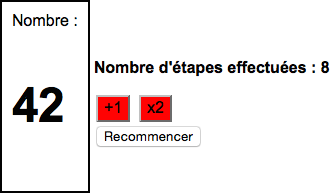
\includegraphics[width=\linewidth]{51-calc}
\caption{\note{An example of exercise of the Castor contest. Contestants had to make 51 using the fewest operations possible among $+$1 and $\times$2. The goal of the exercise is to give an insight to the binary representation of numbers.}}
\label{fig:51}
\end{figure}

\subsection{Simulation Design}

In our experiments, we analyze the effect of \alert{two} parameters: the number of questions asked and the number of skills $K$ of the q-matrices. For both models considered, Rasch and q-matrix, our Castor train dataset was composed of the same 48,939 students, the test dataset containing the remaining 10,000 students. Several implementations of q-matrix were simulated for $K$ values from 1 to 6.

\note{To evaluate the different models throughout the CAT process, we compute for each student of the test dataset the mean error of its predicted performance over the remaining questions, according to the ground truth, and we take the mean value of this mean error over all test students.}

Our implementation is written in Python and R using the packages \texttt{rpy2} for \alert{R bindings in Python}~\cite{Gautier2008}, \texttt{ltm} for latent trait models of IRT~\cite{Rizopoulos2006} and \texttt{catR} for computerized adaptive testing over the \texttt{ltm} package~\cite{MagisRaiche2012}. The code is available on Bitbucket\footnote{\phantom{\url{http://bitbucket.org/jilljenn/qmatrix/}}}. The whole simulation process ran for 4 hours on a \alert{1.3 GHz Intel Core i7}. % TODO Athena

\subsection{Results}

We compared the R implementation of the Rasch model and our implementation of the NIDA q-matrix model for different values of the parameter $K$, the number of columns of the q-matrix. From now on, we will denote them respectively by IRT and Q.

\subsubsection{Algorithm Speed}

\note{Process time of train and test phases is depicted in Table~\ref{tab:time}. IRT has the fastest train phase and the slowest test phase, which is still reasonable given that the values for the test phase were computed over 10,000 students. As expected by our estimation of complexity, the simulation time for Q grows exponentially with $K$; nevertheless, the fact that most time of the simulation is spent on the train phase makes the q-matrix model suitable for adaptive testing.}

\begin{table}
\small\centering\begin{tabular}{@{}ccc@{}}
& Train phase & Test phase\\
\hline
IRT & 1 min 49 s & 4 min 20 s\\%0.499 $\pm$ 0.024 & 0.469 $\pm$ 0.020 & 0.446 $\pm$ 0.015\\
Q $K = 1$ & 2 min 32 s & 7 s\\
Q $K = 2$ & 5 min 24 s & 14 s\\
Q $K = 3$ & 10 min 57 s & 25 s\\ %0.517 $\pm$ 0.016 & 0.470 $\pm$ 0.012 & 0.444 $\pm$ 0.012\\
Q $K = 4$ & 23 min 29 s & 49 s\\ %0.494 $\pm$ 0.015 & 0.459 $\pm$ 0.011 & 0.417 $\pm$ 0.011\\
Q $K = 5$ & 48 min 42 s & 1 min 35 s\\ %\textbf{0.474 $\pm$ 0.014} & 0.433 $\pm$ 0.011 & 0.415 $\pm$ 0.011\\
Q $K = 6$ & 1 h 45 min 3 s & 3 min 14 s %0.482 $\pm$ 0.015 & \textbf{0.425 $\pm$ 0.012} & \textbf{0.403 $\pm$ 0.011}\\
\end{tabular}
\caption{Process time of train and test phases for each algorithm, over all dataset.}
\label{tab:time}
\end{table}

\subsubsection{Performance Evaluation}

 Results are presented in Figure~\ref{fig:castor} and Table~\ref{tab:error} where the best performances are shown in bold. As a reference, 1.0 is the error obtained by the trivial algorithm affecting 1/2 to every probability. \note{The tightness of the confidence intervals allows us to state that IRT performs slightly better than Q for any value of $K$.} % On the SAT dataset, for all reasonable choices of $K$, the q-matrix model outperforms IRT, the q-matrix of $K = 6$ skills being globally the best among all tested ones.

\begin{table}[H]
\small\centering\begin{tabular}{@{}cccc@{}}
& 4 & 10 & 16\\
\hline
%IRT & 0.482 $\pm$ 0.022 & 0.473 $\pm$ 0.017 & 0.456 $\pm$ 0.019\\
%Q $K = 3$ & 0.487 $\pm$ 0.016 & 0.470 $\pm$ 0.017 & 0.435 $\pm$ 0.012\\
%Q $K = 4$ & \textbf{0.455 $\pm$ 0.017} & 0.434 $\pm$ 0.016 & 0.424 $\pm$ 0.016\\
%Q $K = 5$ & 0.481 $\pm$ 0.022 & \textbf{0.399 $\pm$ 0.015} & 0.376 $\pm$ 0.013\\
%Q $K = 6$ & \textbf{0.455 $\pm$ 0.023} & 0.400 $\pm$ 0.015 & \textbf{0.361 $\pm$ 0.015}\\
Q $K = 1$ & 0.508 $\pm$ 0.003 & 0.394 $\pm$ 0.005 & 0.177 $\pm$ 0.011 \\
Q $K = 2$ & 0.514 $\pm$ 0.003 & 0.407 $\pm$ 0.005 & 0.170 $\pm$ 0.013 \\
Q $K = 3$ & 0.520 $\pm$ 0.003 & 0.425 $\pm$ 0.006 & 0.227 $\pm$ 0.015 \\
Q $K = 4$ & 0.514 $\pm$ 0.004 & 0.433 $\pm$ 0.006 & 0.174 $\pm$ 0.014 \\
Q $K = 5$ & 0.510 $\pm$ 0.004 & 0.401 $\pm$ 0.006 & 0.213 $\pm$ 0.016 \\
Q $K = 6$ & 0.518 $\pm$ 0.004 & 0.436 $\pm$ 0.006 & 0.221 $\pm$ 0.016 \\
IRT & \textbf{0.495 $\pm$ 0.003} & \textbf{0.361 $\pm$ 0.005} & \textbf{0.136 $\pm$ 0.012} \\
\end{tabular}
\caption{Mean error of the different algorithms \alert{over} the remaining questions of the 17-question Castor contest, after 4, 10 and 16 questions have been asked.}
\label{tab:error}
\end{table}

\alert{Q algorithms for different values of $K$ seem to have similar mean error, the $K = 6$ one achieving the highest error. A longer skill vector is harder to guess, thus requires more questions.} % TODO

\note{Examples of estimated parameters are shown in Figure~\ref{tab:example}: item difficulties for IRT, binary matrix entries and slip/guess parameters for Q. The corresponding success rates of the student data give an insight to the intrinsic difficulties of the different questions. For example, questions 1 and 13 seem the hardest ones of the test, which is why both of them require all concepts in order to be solved. But question 13 is itself harder than question 1, therefore this results in a higher slip parameter. But high values of slip/guess parameters slow down the determination of the skill vector of the student. This may be responsible for the behavior of Q opposed to IRT.}

%\begin{figure}
%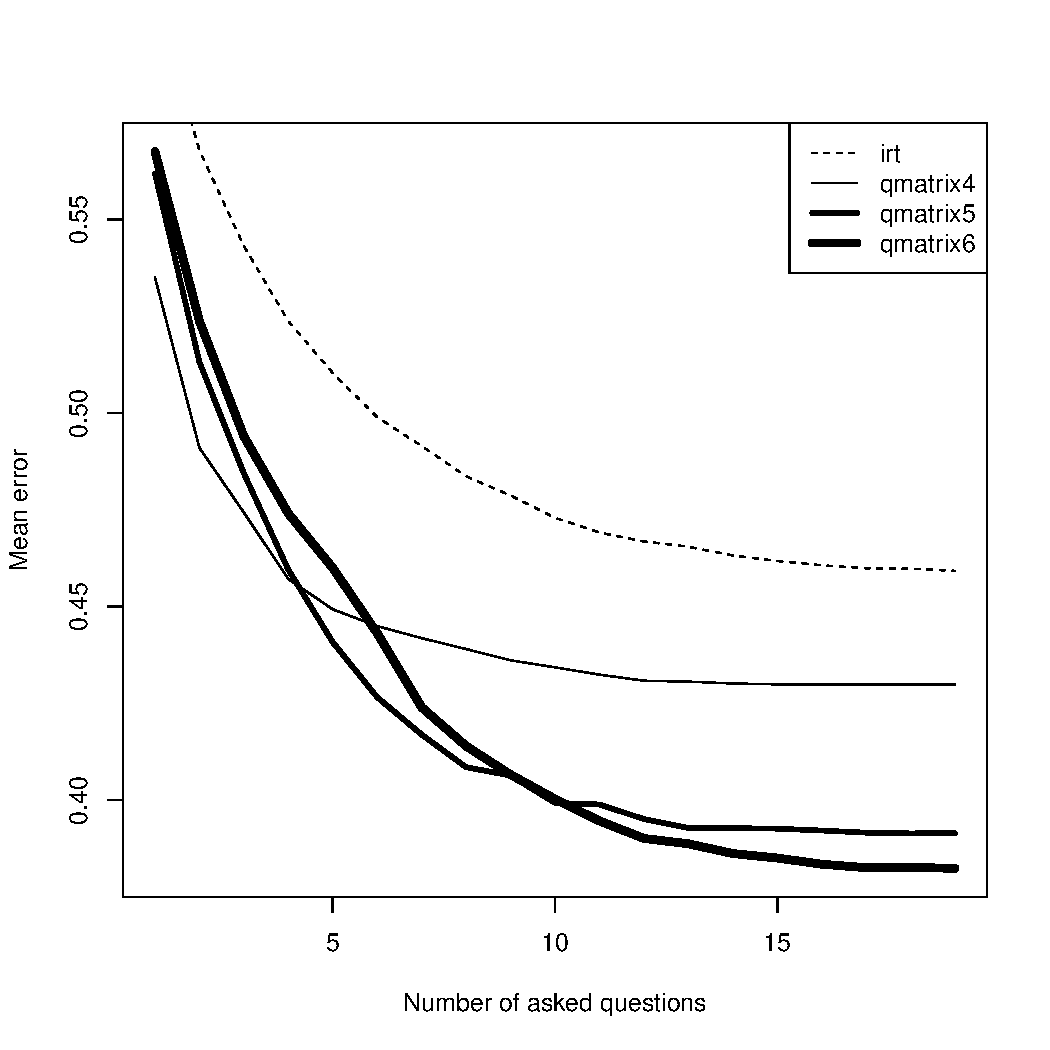
\includegraphics[width=\linewidth]{20-80.pdf}
%\caption{Evolution of the mean error throughout the test, for a train dataset of size 80 and a 20-question test. The dashed curve denotes the IRT model, while the curves of growing thickness denote q-matrices of growing number of columns.}
%\label{fig:1}
%\end{figure}

\begin{figure}
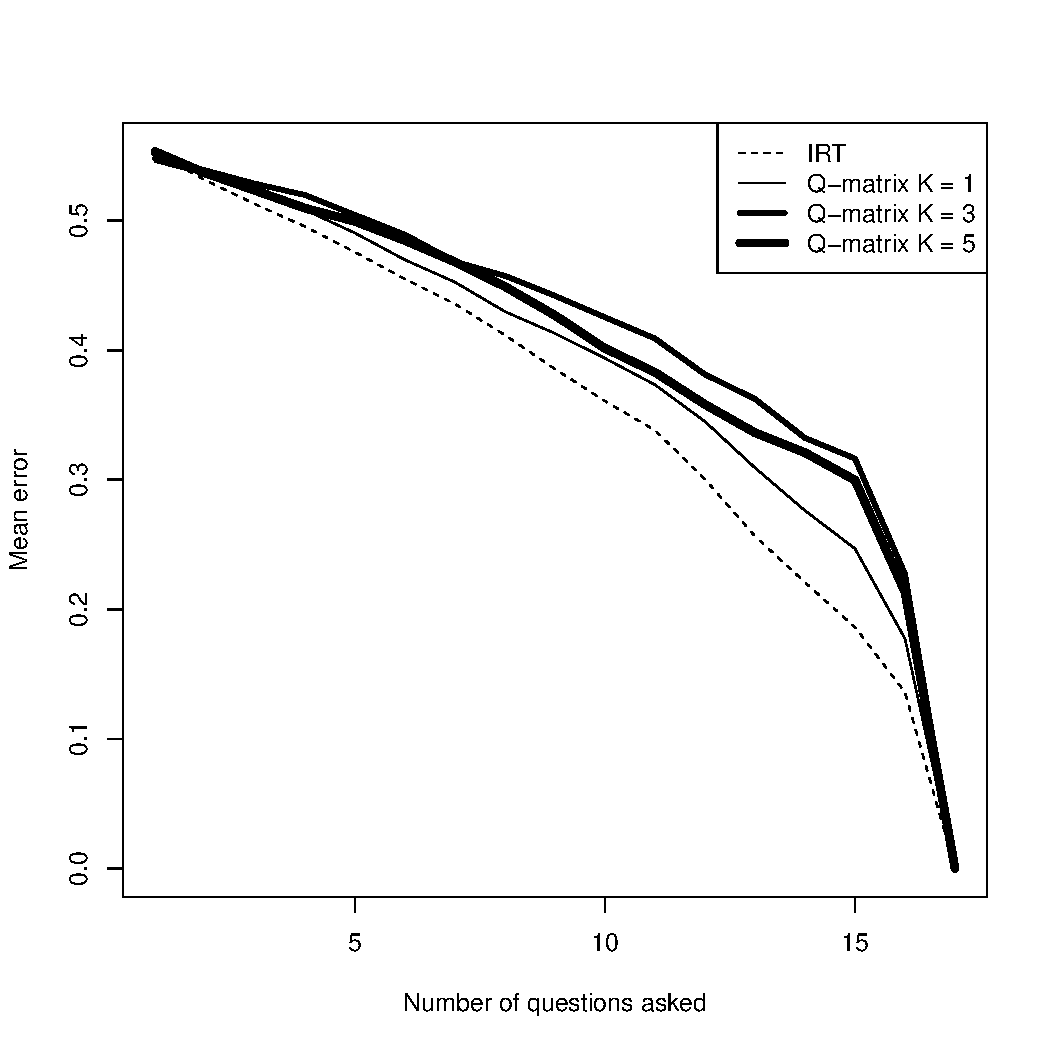
\includegraphics[width=\linewidth]{castor.pdf}
\caption{\note{Evolution of the mean error on the remaining questions after a certain number of questions of the Castor contest have been asked. The dashed curve denotes the IRT model, while the curves of growing thickness denote q-matrices of growing number of columns. IRT performs slightly better.}}
\label{fig:castor}
\end{figure}

\begin{table}
\small\centering\begin{tabular}{c|c|ccccc|c}
\# & IRT difficulty & 	\multicolumn{3}{c}{Q-Matrix} & Guess & Slip & Success\\
\hline
1 & 2.454 & 	1 & 1 & 1 & 0.059 & \textbf{0.645} & 11 \% \\
2 & -1.121 & 	1 & 0 & 0 & \textbf{0.512} & 0.082 & 72 \% \\
3 & -2.015 & 	0 & 0 & 0 & \textbf{0.504} & 0.152 & 85 \% \\
4 & -1.260 & 	0 & 0 & 0 & \textbf{0.504} & 0.254 & 74 \% \\
5 & 0Q2 .932 & 	0 & 0 & 1 & 0.012 & 0.027 & 31 \% \\
6 & -0.080 & 	0 & 1 & 0 & 0.324 & 0.027 & 52 \% \\
7 & 0.111 & 	1 & 1 & 0 & 0.309 & 0.035 & 48 \% \\
8 & 0.442 & 	1 & 0 & 0 & 0.215 & 0.41 & 41 \% \\
9 & 1.062 & 	1 & 1 & 1 & 0.246 & 0.496 & 29 \% \\
10 & 0.858 & 	0 & 1 & 0 & 0.105 & 0.082 & 33 \% \\
11 & 0.878 & 	1 & 0 & 1 & 0.207 & 0.285 & 32 \% \\
12 & -0.056 & 	0 & 1 & 0 & 0.371 & 0.121 & 51 \% \\
13 & 3.533 & 	1 & 1 & 1 & 0.02 & \textbf{0.809} & 4 \% \\
14 & 2.255 & 	1 & 0 & 1 & 0.059 & 0.66 & 12 \% \\
15 & -0.048 & 	1 & 0 & 0 & 0.02 & 0.027 & 51 \% \\
16 & 0.063 & 	1 & 0 & 1 & 0.387 & 0.176 & 49 \% \\
17 & 1.803 & 	1 & 1 & 1 & 0.113 & 0.496 & 18 \%
\end{tabular}
\caption{Example of question parameters for the Rasch model vs. q-matrix $K = 3$ and success rate in the train dataset. The q-matrix model compensates the lack of a difficulty parameter with high values of the slip and guess parameters. Values greater than 0.5 are denoted in bold.}
\label{tab:example}
\end{table}

\section{Discussion and Future Work}

Our studies suggest that the q-matrix model, first designed for cognitive diagnosis, can successfully be used in a context of large-scale assessments, \alert{both in terms of speed and predicting quality}. This model is thus suitable for placement tests, where few questions should be enough to explore at best the examinee's skills. More globally, it can be used for low-stakes testing, but not high-stakes testing, as the first questions chosen by the item selection rule from one student to another. This high item exposure rate was already pointed out in~\cite{Cheng2009}.

%Pay attention to the fact that although the training step is longer for the q-matrix model than the IRT chosen model, the next-item step is several times longer for the IRT model with minimum expected posterior variance criterion than the q-matrix model. Thus, for a given test, once a good q-matrix has been computed in a preprocessing step, the test can be administered in a reasonable time. % Can be linked to the prior.

% On the first hand, the Rasch model tries to guess a one-dimensional geometry for the question data. On the other hand, the q-matrix model allows a directed-acyclic-graph-like structure to comprehend the question data.

\note{Surprisingly, on the Castor dataset, our implementation of the simplest Rasch model performs slightly better than our q-matrix implementations for $K$ from 1 to 6. In order to address this problem, both models should be compared to a more conventional dataset such as a simple calculus test, requiring fewest competences. Also, a better computation of q-matrix using more cutting-edge techniques could lead to other results.} % TODO pas bon

%However, q-matrix being a richer model, it can be prone to overfitting, particularly for greater values of $K$, as highlighted by our results. In addition, the longer convergence time for high values of $K$ can be explained by the fact that guessing a larger skill vector requires more information, therefore more questions. Thus, there is a tradeoff between a large value of $K$ potentially leading to overfitting and smaller ones which could not provide a rich enough model. The optimal value of $K$ may depend on the size of the training set along with the number of questions of the test. Nevertheless, as pointed out in~\cite{Huebner2010}, there have been no systematic studies for cognitive diagnosis models investigating the most suitable number of skills $K$ for a given dataset.

% Finally, while the optimization of the $K$ parameter is important, the sensibility of the results to this parameter is tempered. Indeed, the results for q-matrix with $K = 5$ and $K = 6$ are actually pretty close. % K

% Our results suggest that q-matrix is not very sensitive to the choice of K as long as this K parameters keep being reasonable given the train dataset.

We made no hypothesis at all on the links between questions, \alert{which is why} we got a probability distribution of size $2^K$, slowing down both the train and test phases of Q. Assuming pairwise independence of the skills would lead to $O(K)$ complexity instead of $O(2^K)$, enabling us to explore a wider range of q-matrix sizes. As pointed out in~\cite{Huebner2010}, there have been no systematic studies so far investigating the most suitable number of skills $K$ for a given dataset.

%  Due to limited resources, our simulation was limited to $K \leqslant 6$. Indeed, the most costly part of the process is the training step of the q-matrix, which requires at each iteration a cost exponential in $K$ and a number of iterations increasing with $K$ to obtain convergence towards a local minimum. A better computation of q-matrix using more cutting-edge techniques could have lead to even better results. % TODO insister sur le fait qu'on ne s'est pas concentrés sur le calcul de la Q-matrice

%Our results can extended to other cognitive diagnosis models from the compensatory classes (DINA, etc.~\cite{Desmarais2011}).

%A new direction could be to 

%Please also note that, our item exposure rate is very high as the same first questions are asked. Thus low stakes high stakes

% On another note, our results are produced from a dataset over 4 knowledge fields. It would be interesting to compare IRT-based models and q-matrix models on other real data such as bigger datasets or ones including only one knowledge field.



%We showed that links between questions are worth taking into account, something q-matrices do and IRT does not. For our evaluation, we chose the simplest models from item response theory and cognitive diagnosis, but more complex models such as multidimensional item response theory~\cite{Desmarais2012} or fusion models~\cite{McGlohen2008} should be compared to the NIDA q-matrix model presented here.

% MIRT

% As a finish we would like to draw a link between Elo systems and IRT because the probability of winning only depends on the difference between Elo values while the probability of answering correctly. 

% Chess stuff.

%Add a last column to q-matrix

%No study has been done yet over the number of skills.

%Outperforms on both simulated data and real data.

\section{Acknowledgements}

We thank Chia-Tche Chang, Le Thanh Dung Nguyen and especially Antoine Amarilli for their valuable comments.

%\bibliographystyle{abbrv}
\bibliographystyle{plain}
\bibliography{sigproc}  % sigproc.bib is the name of the Bibliography in this case
% You must have a proper ".bib" file
%  and remember to run:
% latex bibtex latex latex
% to resolve all references
%
% ACM needs 'a single self-contained file'!
%
%APPENDICES are optional
%\balancecolumns
%\appendix
%Appendix A
%\section{If I have something more to say}

%\balancecolumns % GM June 2007
% That's all folks!
\end{document}
